\documentclass[a4paper,12pt,oneside]{skripsi}

\usepackage[bahasa]{babel}
\usepackage[T1]{fontenc}
\usepackage{mathptmx}
\usepackage[latin1]{inputenc}
\setcounter{secnumdepth}{3}
\setcounter{tocdepth}{3}
\usepackage{array}
\usepackage{longtable}
\usepackage{graphicx}
\usepackage{setspace}
\usepackage{multind}
\usepackage{rotating} %for rotate/sideway text
\usepackage{subfig} %for make floating sub-figure
\usepackage[top=4cm, bottom=3cm, left=4cm, right=3cm]{geometry}

%\makeindex{subject}
\centerchapter
\makeatletter
\doublespacing
\makeatother
\parindent 3.0em

%===================================================================
% \setlength{\textwidth}{15.0cm}
% \setlength{\evensidemargin}{2.5cm} % outer/right margin
% % \setlength{\topmargin}{0.3cm}    % top margin
% \setlength{\footskip}{2.5cm}       % distance between text and foot
% \setlength{\textheight}{\paperheight}
% \addtolength{\textheight}{-\topmargin}
% \addtolength{\textheight}{-\headheight}
% \addtolength{\textheight}{-\headsep}
% \addtolength{\textheight}{-\footskip}
% \addtolength{\textheight}{-4cm}   % bottom margin
%==============================================================================
\tolerance=1
\emergencystretch=\maxdimen
\hyphenpenalty=10000
\hbadness=10000

\addto\captionsbahasa{
  \renewcommand{\contentsname}{DAFTAR ISI} 
  \renewcommand{\listfigurename}{DAFTAR GAMBAR}
  \renewcommand{\listtablename}{DAFTAR TABEL}
  \renewcommand{\chaptername}{BAB}
  \renewcommand{\chaptername}{BAB}
  \renewcommand{\bibname}{DAFTAR PUSTAKA}
}


\begin{document}

\nocite{*}
%#start bagian administrasi #==================================================
% bagian muka sebelum isi, umumnya halaman administrasi, kalau tidak digunakan
% dapat diberikan tanda % didepannya

%cover
\pagestyle{empty}
\pagenumbering{roman}
\setcounter{page}{1}
\newpage

\addcontentsline{toc}{chapter}{HALAMAN JUDUL}

\begin{center}

\bfseries

{\Large UNIVERSITAS GUNADARMA}\\
{\Large FAKULTAS TEKNOLOGI INDUSTRI}\\

\vspace{1.0cm}

\begin{figure}[h]
  \begin{center}
    \includegraphics[scale=4.5]{gambar/LogoGunadarma.jpg}
  \end{center}
\end{figure}

{\large ESTIMASI POSE TIGA DIMENSI DARI GAMBAR MONOKULER MENGGUNAKAN DEEP NEURAL NETWORK}

\vspace{1.5cm}

\begin{tabular}{|c|}
  \hline
  Disusun oleh: \\
  \begin{tabular}{ll}
  Nama& : Denilson \\[-5pt]
  NPM& : 51416815 \\[-5pt]
  Jurusan& : Teknik Informatika \\[-5pt]
  Pembimbing& : Dr. Dharmayanti, ST., MMSI.\\
  \end{tabular}\\
  \hline
\end{tabular}

\end{center}

\vspace{1.5cm}

\begin{center}
\bfseries
Diajukan Guna Melengkapi Sebagian Syarat \\
Dalam Mencapai Gelar Sarjana Strata Satu (S1)\\

Depok\\
2020 %DIGANTI TAHUN PENULISAN SKRIPSI
\end{center}



%halaman lembar pengesahan, abstraksi, kata pengantar
\pagestyle{plain}
\pagenumbering{roman}
\setcounter{page}{2} %nilai halaman utk awal dari abstrak s/d ucapan terimakasih dlm romawi
\newpage
\addcontentsline{toc}{chapter}{LEMBAR PENGESAHAN}
\begin{center}
    {\large \bf \centering LEMBAR PENGESAHAN}

    \vspace{0.75cm}

    {\bf Komisi Pembimbing}

    \vspace{0.5cm}

    \begin{tabular}{|c|c|c|}
        \hline
        No & Nama                        & Kedudukan                 \\
        \hline

        1  & Dr. Dharmayanti, ST., MMSI. & Ketua                     \\
        \hline

        2  & DIGANTI NAMA PENGUJI 2      & DIGANTI JABATAN PENGUJI 2 \\
        \hline
        3  & DIGANTI NAMA PENGUJI 3      & DIGANTI JABATAN PENGUJI 3 \\
        \hline
    \end{tabular}

    \vspace{0.1cm}
    \begin{flushright}
        {Tanggal Sidang : tgl bln thn}
    \end{flushright}

    \vspace{0.5cm}

    {\bf Panitia Ujian}

    \vspace{0.5cm}

    \begin{tabular}{|c|c|c|}
        \hline
        No & Nama                   & Kedudukan                 \\
        \hline

        1  & DIGANTI NAMA PENGUJI 1 & DIGANTI JABATAN PENGUJI 1 \\
        \hline

        2  & DIGANTI NAMA PENGUJI 2 & DIGANTI JABATAN PENGUJI 2 \\
        \hline
        3  & DIGANTI NAMA PENGUJI 3 & DIGANTI JABATAN PENGUJI 3 \\
        \hline
        4  & DIGANTI NAMA PENGUJI 4 & DIGANTI JABATAN PENGUJI 4 \\
        \hline
        5  & DIGANTI NAMA PENGUJI 5 & DIGANTI JABATAN PENGUJI 5 \\
        \hline
    \end{tabular}

    \vspace{0.1cm}
    \begin{flushright}
        {Tanggal Lulus : tgl bln thn}
    \end{flushright}

    {\bf Mengetahui,}

    \vspace{0.5cm}

    {Pembimbing~ \hspace{5.0cm} ~Bagian Sidang Sarjana}%

    \vspace{1.5cm}

    {(Dr. Dharmayanti, ST., MMSI.)~ \hfill ~(NAMA BAGIAN SARJANA)}%


\end{center}
% menggabungkan file lembar pengesahan

\newpage %Abstract
\addcontentsline{toc}{chapter}{ABSTRAKSI}
\begin{center}
    \begin{large}\textbf{ABSTRAKSI}\end{large}
\end{center}

\vspace{5mm}

\noindent Denilson, 51416815 \\
ESTIMASI POSE TIGA DIMENSI DARI GAMBAR MONOKULER MENGGUNAKAN DEEP NEURAL NETWORK\\
Tugas Akhir. Jurusan Teknik Informatika, Fakultas Teknologi Industri, \\
Universitas Gunadarma, 2020\\
Kata Kunci: Estimasi Pose, Gambar Monokuler, Jaringan Saraf Tiruan, Pemelajaran Dalam, Visi Komputer\\
\noindent (xiv + 38 + lampiran)\\

\setstretch{1.0}
Perkembangan teknologi digital yang pesat baik pada aplikasi atau ilmu pengetahuan dapat
manghasilkan rekam jejak digital yang bermanfaat. Jumlah data digital yang tersedia sangat
banyak dan diprediksi akan semakin bertambah. Salah satu penggunaan data adalah membuat
suatu fungsi pemetaan yang mencari korelasi antara suatu domain ke domain lainnya dengan
menggunakan data terkait sebagai acuan dasar. Data digital berbentuk rangkaian gambar atau video
merupakan data yang bersifat laten yang berarti data tersebut memiliki informasi semantik yang
tersembunyi. Penelitian ini membahas pembuatan sebuah fungsi yang memetakan gambar dua dimensi
terhadap titik kunci pose tiga dimensi yang bersifat laten menggunakan permodelan
\textit{deep neural network}. Perangkat lunak yang dibangun dengan pemrosesan data,
perancangan arsitektur model, pemelajaran model secara mandiri, dan menampilkan visualisasi
penggunaan model. Arsitektur model yang digunakan terdiri dari beberapa blok \textit{residual network}
yang menambahkan \textit{input} terhadap \textit{output} masing-masing blok. Hasil dari uji coba menjelaskan
bahwa teori dan data yang dipakai benar dan penggunaan aplikasi terhadap data baru berjalan
sesuai prediksi.\\


\setstretch{1.5}
\noindent Daftar Pustaka (1986-2020)
% menggabungkan file abstraksi

%menggabungkan file CV atau riwayat hidup ringkas
%\include{cv}
\newpage %Acknowledgment
\addcontentsline{toc}{chapter}{KATA PENGANTAR}
\begin{center}
\begin{large}\textbf{KATA PENGANTAR}\\\end{large}
\end{center}
\vspace{5mm}


Segala puji dan syukur penulis ucapkan ke hadirat Tuhan Yang Maha Esa yang telah memberikan berkat, 
anugerah dan karunia yang melimpah, sehingga penulis dapat menyelesaikan Tugas Akhir ini pada waktu 
yang telah ditentukan.

Tugas Akhir ini disusun guna melengkapi sebagian syarat untuk memperoleh gelar Sarjana Teknik 
Informatika Universitas Gunadarma. Adapun judul Tugas Akhir ini adalah "Estimasi Pose Tiga Dimensi
Dari Gambar Monokuler Menggunakan Deep Neural Network".

Walaupun banyak kesulitan yang penulis harus hadapi ketika menyusun Tugas Akhir ini, namun berkat 
bantuan dan dorongan dari berbagai pihak, akhirnya Tugas Akhir ini dapat diselesaikan dengan baik. 
Untuk itu penulis tidak lupa mengucapkan terima kasih kepada:

\begin{enumerate}
  \item Ibu Prof. E. S. Margianti, SE, MM selaku rektor Universitas Gunadarma
  \item ............ selaku Dekan Fakultas ........ Universitas Gunadarma
  \item ............ selaku Ketua Jurusan ..............
  \item ............ selaku Bagian Sidang Sarjana
  \item Ibu Dr. Dharmayanti, ST., MMSI sebagai pembimbing penulis yang ditengah-tengah kesibukannya 
  telah membimbing penulis sehingga penulisan ini dapat diselesaikan.
  \item Keluarga yang selalu mendukung dan terus memberikan motivasi.
  \item Semua pihak yang terlibat dalam membantu penyelesaian Tugas Akhir ini.

\end{enumerate}

Sebagai manusia biasa yang tak luput dari kesalahan, maka penulis meminta maaf atas segala 
kekurangan dan keterbatasan dalam penyusunan Tugas Akhir ini. Penulis sadari bahwa penulisan ini 
masih jauh dari sempurna, disebabkan karena berbagai keterbatasan yang penulis miliki. Untuk itu 
penulis mengharapkan kritik dan saran yang bersifat membangun untuk menjadi perbaikan di masa yang 
akan datang.

Akhir kata, penulis berharap penulisan ini dapat bermanfaat bagi kita semua dan bagi penulis 
pribadi khususnya, serta dapat digunakan sebagaimana mestinya.


\vspace{0.5 cm}
\begin{flushright}
Depok, April 2020

\vspace{2 cm}
Penulis
\end{flushright}% mengabungkan file kata pengantar

%# akhir bagian administrasi # ==========================================

% #mulai membuat daftar isi, daftar gambar dan  daftar tabel # ==========
%\setcounter{page}{8} %set nilai halaman sesuai urutannya

% membuat daftar isi
\tableofcontents{}
\addcontentsline{toc}{chapter}{DAFTAR ISI}

%membuat daftar gambar
\listoffigures
\addcontentsline{toc}{chapter}{DAFTAR GAMBAR}%masih masalah

%% membuat daftar tabel
\listoftables
\addcontentsline{toc}{chapter}{DAFTAR TABEL}

%\newpage %lampiran
\addcontentsline{toc}{chapter}{DAFTAR LAMPIRAN}
\begin{center}
    \begin{large}\textbf{DAFTAR LAMPIRAN}\\\end{large}
\end{center}
\vspace{5mm}
\noindent Lampiran 1: Kelas Dataset
. . . . . . . . . . . . . . . . . . . . . . . . . . . . . . . . . . . . . . L1

\noindent Lampiran 2: Kelas ResLinear
. . . . . . . . . . . . . . . . . . . . . . . . . . . . . . . . . . . . L1

\noindent Lampiran 3: Arsitektur Model
. . . . . . . . . . . . . . . . . . . . . . . . . . . . . . . . . . . .L1

\noindent Lampiran 4: Options
. . . . . . . . . . . . . . . . . . . . . . . . . . . . . . . . . . . . . . . . . . L2

\noindent Lampiran 5: Pemuatan Data
. . . . . . . . . . . . . . . . . . . . . . . . . . . . . . . . . . . . . L2

\noindent Lampiran 6: Instansiasi Dataset dan DataLoader
. . . . . . . . . . . . . . . . . . . . . . .L2

\noindent Lampiran 7: Algoritma Pelatihan
. . . . . . . . . . . . . . . . . . . . . . . . . . . . . . . . . L2

\noindent Lampiran 8: Algoritma Validasi
. . . . . . . . . . . . . . . . . . . . . . . . . . . . . . . . . . L2

\noindent Lampiran 9: Instansiasi Model
. . . . . . . . . . . . . . . . . . . . . . . . . . . . . . . . . . . L2

\noindent Lampiran 10: Visualisasi Titik Kunci
. . . . . . . . . . . . . . . . . . . . . . . . . . . . . . .L3

\noindent Lampiran 11: Visualisasi Inferensi
. . . . . . . . . . . . . . . . . . . . . . . . . . . . . . . . L3

\noindent Lampiran 12: Plot Grafik
. . . . . . . . . . . . . . . . . . . . . . . . . . . . . . . . . . . . . . . L3

% #akhir membuat daftar isi, daftar gambar dan  daftar tabel # ==========

% # mulai bagian isi # ==================================================

\newpage
\pagestyle{headings}
\pagenumbering{arabic} % jenis huruf arabic
\setcounter{page}{1} %mulai dari halaman 1



\chapter{PENDAHULUAN}
\label{cha:1-Pendahuluan}

\section{Latar Belakang}
\label{sec:1-LatarBelakang}

Bagian ini menceritakan latar belakang dari penelitian.
Bagian ini menceritakan latar belakang dari penelitian.
Bagian ini menceritakan latar belakang dari penelitian.
Bagian ini menceritakan latar belakang dari penelitian.
Bagian ini menceritakan latar belakang dari penelitian.
Bagian ini menceritakan latar belakang dari penelitian.
Bagian ini menceritakan latar belakang dari penelitian.
Bagian ini menceritakan latar belakang dari penelitian.
Bagian ini menceritakan latar belakang dari penelitian.
Bagian ini menceritakan latar belakang dari penelitian.
Bagian ini menceritakan latar belakang dari penelitian.
Bagian ini menceritakan latar belakang dari penelitian.
Bagian ini menceritakan latar belakang dari penelitian.
Bagian ini menceritakan latar belakang dari penelitian.
Bagian ini menceritakan latar belakang dari penelitian.


\section{Batasan dan Tujuan}
\label{sec:1-BatasTujuan}

Bagian ini menceritakan tentang :
\begin{itemize}
\item Batasan penelitian beserta alasannya.
\item Definisi permasalahan dari penelitian
\item Tujuan umum dan khusus dari penelitian
\end{itemize}

 
\begin{figure}[tb]
\vspace{-0.3cm}
%\rule{\columnwidth}{0.1pt}
\begin{center}
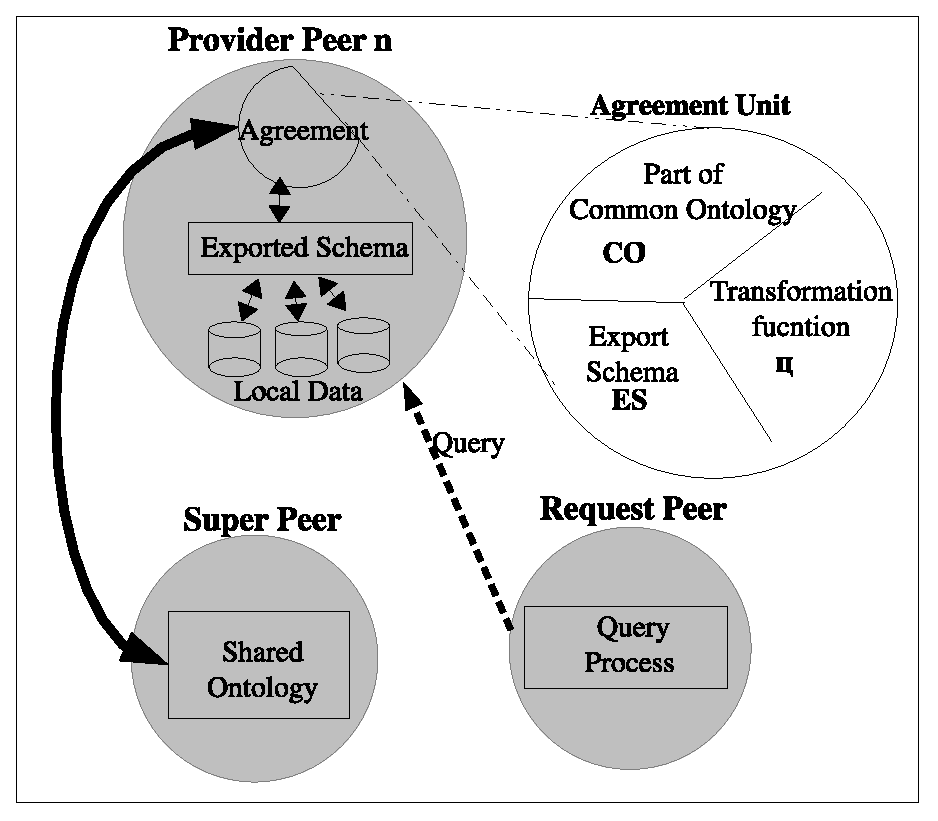
\includegraphics[width=0.7\columnwidth]{bab1/ContohGbr1_1.eps}
\end{center}
\vspace{-0.5cm}
%\rule{\columnwidth}{0.1pt}
\caption{\small Contoh 1.1 untuk menampilkan gambar \label{fig:1-contoh1.1}}
\end{figure}


\section{Kontribusi}
\label{sec:1-Kontribusi}
Menjelaskan kontribusi utama dari hasil penelitian.

\textit{\textbf{Ini mendemonstrasikan fungsi label untuk mengacu kepada sebuah gambar. Lihat gambar \ref{fig:1-contoh1.1} sebagai contoh awal. Contoh referensi lihat referensi \cite{Sheth:b}}
} %Bab 1.Pendahuluan



\chapter{TINJAUAN PUSTAKA}
\label{cha:2-TinjauanPustaka}

\section{Teorema Penaksiran Universal}
\label{sec:2-TeoremaPenaksiranUniversal}

Teorema penaksiran universal atau \textit{universal approximation theorem} menyatakan bahwa sebuah
model jaringan \textit{feed-forward} dapat membentuk fungsi apapun secara subjektif. Sebuah model
jaringan saraf tiruan dibentuk dari serangkaian lapisan yang didalamnya terdapat deretan sel saraf
atau \textit{neuron} dengan kuantitas tertentu. Semakin panjang rangkaian lapisan yang tersedia,
maka semakin banyak saraf yang tersedia sehingga dapat memetakan fungsi yang sulit.
Model jaringan yang memiliki banyak saraf dapat mempelajari pola-pola yang ada dari satu
domain ke domain lainnya~\cite{2016arXiv160100013G}.

Teorema penaksiran universal memiliki dua sifat yang dikategorikan berdasarkan pemanfaatannya dalam
melakukan pemelajaran mesin. Sifat pertama adalah suatu model jaringan saraf tiruan dapat
memperkirakan suatu fungsi dengan batasan-batasan tertentu sesuai dengan fungsi aktivasi pada
lapisan terakhir. Sifat kedua adalah sebuah fungsi kontinu dengan jumlah variabel sembarang dapat
ditiru oleh sebuah jaringan saraf tiruan dengan jumlah yang sembarang~\cite{2019arXiv191003344K}.

\section{Jaringan Saraf}
\label{sec:2-JaringanSaraf}

Otak manusia terdiri dari kumpulan sel saraf yang saling terkoneksi satu sama lain. Sebuah sel saraf
adalah sel yang dapat memproses dan mengantarkan informasi apabila dirangsang dengan tegangan
elektrokimia. Sel-sel saraf tidak pernah memperbanyak dirinya dan tidak digantikan apabila ada yang
rusak. Jumlah sel saraf yang terdapat dalam otak manusia diperkirakan sebanyak satu miliar. Setiap
sel saraf diperkirakan berkoneksi dengan sepuluh ribu sel saraf lainnya melalui sinapsis yang
berarti otak manusia beroperasi seperti prosesor dengan kecepatan satu triliun bit per
detik~\cite{10.3389/neuro.09.031.2009}.

\begin{figure}[htbp]
    \begin{center}
        \fbox{\includegraphics[scale=1.0]{bab2/gambar/jaringansaraf.jpg}}
    \end{center}
    \vspace{-20pt}
    \captionsetup{labelfont=bf, textfont=bf}
    \caption{Ilustrasi Jaringan Saraf Manusia}
    \vspace{-10pt}
    \captionsetup{labelfont=md, textfont=md}
    % \caption*{Sumber: https://upload.wikimedia.org/wikipedia/commons/b/b5/Neuron.svg}
    % \caption*{Sumber: Zhang (2019)}
    \label{fig:jaringansaraf}
\end{figure}

Bentuk sel saraf sangat bervariasi dengan berbagai ukuran, bentuk, dan sifat elektrokimianya. Sebuah
sel saraf memiliki badan yang terdiri dari beberapa struktur penting meliputi \textit{soma},
\textit{dendrites}, \textit{axon}, dan \textit{synapses} seperti pada gambar~\ref{fig:selsaraf}.
Sebuah sel saraf akan menerima beberapa masukkan melalui \textit{synapses}, memproses inputan
tersebut melewati \textit{dendrites}, kemudian diteruskan melalui \textit{soma}, dan diberikan
kepada sel saraf lainnya melalui \textit{axon}~\cite{2019arXiv190601703Z}.

\begin{figure}[htbp]
    \begin{center}
        \fbox{\includegraphics[scale=1.0]{bab2/gambar/selsaraf.jpg}}
    \end{center}
    \vspace{-20pt}
    \captionsetup{labelfont=bf, textfont=bf}
    \caption{Ilustrasi Sel Saraf Manusia}
    \vspace{-10pt}
    \captionsetup{labelfont=md, textfont=md}
    % \caption*{Sumber: https://upload.wikimedia.org/wikipedia/commons/b/b5/Neuron.svg}
    % \caption*{Sumber: Zhang (2019)}
    \label{fig:selsaraf}
\end{figure}

\section{Jaringan Saraf Tiruan}
\label{sec:2-JaringanSarafTiruan}

Jaringan Saraf Tiruan adalah sistem komputasi yang cara kerjanya menyerupai jaringan saraf pada otak
makhluk hidup. Tidak seperti pemrograman secara konvensional, sebuah jaringan saraf tiruan dapat
memodelkan fungsi sembarang yang tingkat kesulitannya sesuai dengan jumlah koneksi yang ada. Sama
seperti jaringan saraf asli, sebuah saraf tiruan juga menerima banyak masukkan dari saraf lainnya
kemudian dioperasikan dengan bobot yang terkadung pada sel tersebut dan akhirnya diteruskan ke sel
berikutnya. Jaringan saraf umumnya dibentuk kedalam beberapa lapisan seperti pada
gambar~\ref{fig:jaringansaraftiruan}~\cite{croann}.

\begin{figure}[htbp]
    \begin{center}
        \fbox{\includegraphics[scale=1.0]{bab2/gambar/jaringansaraftiruan.jpg}}
    \end{center}
    \vspace{-20pt}
    \captionsetup{labelfont=bf, textfont=bf}
    \caption{Ilustrasi Jaringan Saraf Tiruan}
    \vspace{-10pt}
    \captionsetup{labelfont=md, textfont=md}
    % \caption*{Sumber: https://upload.wikimedia.org/wikipedia/commons/b/b5/Neuron.svg}
    % \caption*{Sumber: Zhang (2019)}
    \label{fig:jaringansaraftiruan}
\end{figure}

Sebuah sel saraf saraf dapat dibagi menjadi empat bagian yang meliputi masukkan, bobot, fungsi
transfer atau aktivasi, dan keluaran. Jumlah masukkan pada suatu sel saraf tiruan berjumlah sebanyak
output dari sel-sel yang berada pada layer sebelumnya. Bobot sel adalah nilai numerik yang menjadi
identitas dari sel yang merupakan hasil penyesuaian dari proses latihan. Fungsi aktivasi adalah
sebuah fungsi menerima hasil operasi antara bobot dan masukkan. Keluaran merupakan hasil dari sel
yang diteruskan ke lapisan selanjutnya. Ilustrasi sebuah sel saraf tiruan dapat dilihat pada gambar
~\ref{fig:saraftiruan}~\cite{Sharma2012ACS}.

\begin{figure}[htbp]
    \begin{center}
        \fbox{\includegraphics[scale=1.0]{bab2/gambar/saraftiruan.jpg}}
    \end{center}
    \vspace{-20pt}
    \captionsetup{labelfont=bf, textfont=bf}
    \caption{Ilustrasi Sel Saraf Tiruan}
    \vspace{-10pt}
    \captionsetup{labelfont=md, textfont=md}
    % \caption*{Sumber: https://upload.wikimedia.org/wikipedia/commons/b/b5/Neuron.svg}
    % \caption*{Sumber: Zhang (2019)}
    \label{fig:saraftiruan}
\end{figure}

\section{Fungsi Aktivasi}
\label{sec:2-FungsiAktivasi}

Fungsi aktivasi pada sel saraf tiruan berfungsi untuk mengkonversi hasil operasi matriks antara
masukkan dan bobot sebuah sel dari sistem linier ke sistem nonlinier. Konversi nilai ini dilakukan
agar setiap sel mengambil perannya pada saat proses pelatihan model. Beberapa fungsi aktivasi yang
dipakai pada umumnya adalah \textit{Sigmoid}, \textit{ReLU}, \textit{Tanh}, dan \textit{Softmax}
~\cite{2014arXiv1412.6830A}.

\textit{Rectified Linear Unit} adalah fungsi aktivasi yang paling umum digunakan dalam aplikasi
jaringan saraf tiruan. Fungsi aktivasi \textit{ReLU} membatasi nilai masukkannya dimana nilai yang
kurang dari nol akan diubah menjadi nol~\cite{Hinton_rectifiedlinear, 2018arXiv181103378N}.
Persamaan fungsi aktivasi \textit{Rectified Linear Unit} dapat dilihat seperti pada persamaan dibawah.

\begin{equation*}
    \;f(x)=\;max\left(0,x\right)=\;\left\{\begin{array}{l}x_{i,\;}\;\;if\;x_i\;\geq\;0\\0,\;\;\;\;if\;x_i<\;0\;\;\end{array}\right.\;\;
\end{equation*}

\begin{figure}[htbp]
    \begin{center}
        \fbox{\includegraphics[scale=1.0]{bab2/gambar/relu.png}}
    \end{center}
    \vspace{-20pt}
    \captionsetup{labelfont=bf, textfont=bf}
    \caption{\textit{Rectified Linear Unit}}
    \vspace{-10pt}
    \captionsetup{labelfont=md, textfont=md}
    % \caption*{Sumber: https://upload.wikimedia.org/wikipedia/commons/b/b5/Neuron.svg}
    % \caption*{Sumber: Zhang (2019)}
    \label{fig:relu}
\end{figure}

\section{Residual Network}
\label{sec:2-ResidualNetwork}

\textit{Residual Network} atau \textit{ResNet} merupakan model jaringan saraf tiruan yang menggunakan \textit{residual block}
sebagai dasar dari setiap lapisan. Sebuah \textit{residual block} merupakan sebuah arsitektur jaringan
saraf tiruan kecil yang terdiri dari beberapa lapisan. Setiap blok akan menjumlahkan masukkan dan
keluarannya sehingga layer di dalam suatu blok hanya menambahkan pola-pola yang dipelajari. Hal ini
memungkinkan \textit{ResNet} untuk memiliki jumlah blok yang sangat banyak sehingga dapat memetakan
suatu fungsi sembarang yang sulit sesuai dengan teorema penaksiran universal~\cite{2015arXiv151203385H}.
Jenis-jenis \textit{residual block} dapat dilihat pada gambar~\ref{fig:resblock}.

\begin{figure}[htbp]
    \begin{center}
        \fbox{\includegraphics[scale=1.0]{bab2/gambar/resnet.jpg}}
    \end{center}
    \vspace{-20pt}
    \captionsetup{labelfont=bf, textfont=bf}
    \caption{\textit{\textit{Residual Block}}}
    \vspace{-10pt}
    \captionsetup{labelfont=md, textfont=md}
    % \caption*{Sumber: https://upload.wikimedia.org/wikipedia/commons/b/b5/Neuron.svg}
    % \caption*{Sumber: Zhang (2019)}
    \label{fig:resblock}
\end{figure}

\section{Optimisasi Model}
\label{sec:2-OptimisasiModel}

Algoritma optimisasi model yang paling populer dalam melakukan pelatihan model \textit{deep learning}
adalah \textit{gradient descent}. \textit{Gradient descent} meminimalisir selisih antara prediksi
model dan target sebenarnya dengan merubah bobot-bobot yang terdapat dalam model. Nilai bobot yang
ditambahkan berbanding terbalik dengan gradien hasil fungsi kesalahan terhadap masing-masing bobot.
Proses optimisasi dilakukan dengan melakukan \textit{forward-pass} dan \textit{backpropagation} yang
melibatkan beberapa elemen seperti \textit{learning rate}, \textit{optimizer},
dan \textit{loss function}. Tujuannya adalah untuk mencapai titik optimal pada sebuah bidang berdasarkan
hasil dari \textit{loss function}~\cite{2016arXiv160100013G}. Ilustrasi titik optimal digambarkan
pada gambar~\ref{fig:gradientdescent}.

\begin{figure}[htbp]
    \begin{center}
        \fbox{\includegraphics[scale=1.0]{bab2/gambar/gradientdescent.jpg}}
    \end{center}
    \vspace{-20pt}
    \captionsetup{labelfont=bf, textfont=bf}
    \caption{\textit{\textit{Gradient Descent}}}
    \vspace{-10pt}
    \captionsetup{labelfont=md, textfont=md}
    % \caption*{Sumber: https://upload.wikimedia.org/wikipedia/commons/b/b5/Neuron.svg}
    % \caption*{Sumber: Zhang (2019)}
    \label{fig:gradientdescent}
\end{figure}

lr, adam, loss function

\section{Estimasi Pose Dua Dimensi}
\label{sec:2-EstimasiPoseDuaDimensi}
citasi~\cite{8765346}

\section{Estimasi Pose Tiga Dimensi}
\label{sec:2-EstimasiPoseTigaDimensi}

citasi~\cite{martinez_2017_3dbaseline}

\section{PyTorch}
\label{sec:2-PyTorch}

pytorch dynamic graph

\begin{table}[htbp]
    \captionsetup{labelfont=bf, textfont=bf}
    \caption{Sebuah tabel}
    \vspace{-20pt}
    \begin{center}
        \begin{tabular}{| l c r |}
            \hline
            1 & 2 & 3 \\
            4 & 5 & 6 \\
            7 & 8 & 9 \\
            \hline
        \end{tabular}
    \end{center}
    \vspace{-10pt}
    \captionsetup{labelfont=md, textfont=md}
    \caption*{Sumber: Bego Lu}
\end{table}

 %Bab 2.Tinjauan Pustaka


\chapter{PENDEKATAN}
\label{cha:3-Pendekatan}

\section{Gambaran Umum} \label{sec:3-GambaranUmum}

Penelitian ini membahas pemanfaatan data gambar dalam melakukan pelatihan model
\textit{deep neural network}

\section{Kerangka Penelitian} \label{sec:3-KerangkaPenelitian}

\section{Perancangan Aplikasi} \label{sec:3-PerancanganAplikasi}

\subsection{Skema Penerapan Aplikasi}

\subsection{Skema Pelatihan Model}

\section{Analisis Data} \label{sec:3-AnalisisData}

\subsection{Pra-Pemrosesan Data}

\subsection{Definisi Titik Kunci}
COCO Keypoints, Custom Keypoints

\section{Pembuatan Model} \label{sec:3-PerancanganModel}
\subsection{Model A}
\subsection{Model B}
\subsection{Model C}

\section{Pelatihan Model} \label{sec:3-PelatihanModel}

\begin{table}[htbp]
    \captionsetup{labelfont=bf, textfont=bf}
    \caption{Sebuah tabel}
    \vspace{-20pt}
    \begin{center}
        \begin{tabular}{| l c r |}
            \hline
            1 & 2 & 3 \\
            4 & 5 & 6 \\
            7 & 8 & 9 \\
            \hline
        \end{tabular}
    \end{center}
    \vspace{-10pt}
    \captionsetup{labelfont=md, textfont=md}
    % \caption*{Sumber: Bego Lu}
\end{table} %Bab 3.Pendekatan

\chapter{HASIL DAN PEMBAHASAN} \label{cha:4-HasilDanPembahasan}

\section{Hasil Pemelajaran Model} \label{sec:4-PersiapanPengujian}

Pemelajaran model yang dilakukan selama sepuluh \textit{epochs} menunjukkan bahwa kesalahan model
dalam mengestimasi pose tiga dimensi berkurang dalam setiap \textit{epoch}. \text{Learning rate}
yang dibagi dua dalam setiap \textit{epoch} mempengaruhi pemelajaran model dimana penyesuaian model
semakin teliti. Adaptasi bobot model terjadi secara drastis pada \textit{epoch} 0 sampai dengan
\textit{epoch} 3. \textit{Epoch} 4 dan seterusnya menggunakan \textit{learning rate} yang semakin
kecil sehingga model semakin teliti dalam melakukan adaptasi. Grafik pemelajaran model dapat dilihat
pada gambar~\ref{fig:pelatihan}.

\begin{figure}[htbp]
    \begin{center}
        \fbox{\includegraphics[width=11.9cm]{bab4/gambar/pelatihan.jpg}}
    \end{center}
    \vspace{-20pt}
    \captionsetup{labelfont=bf, textfont=bf}
    \caption{Grafik Pemelajaran Model}
    \vspace{-10pt}
    \captionsetup{labelfont=md, textfont=md}
    % \caption*{Sumber: sumber}
    % \caption*{Sumber: nama(2019)}
    \label{fig:pelatihan}
\end{figure}

\section{Analisis Uji Coba Aplikasi} \label{sec:4-PersiapanPengujian}

Inferensi yang bagus akan terjadi apabila langkah-langkah pada tahapan uji coba tidak mengalami
kesalahan. Kualitas gambar dan pose yang tidak cacat juga mempengaruhi proses dari awal hingga akhir.
Prapemrosesan gambar pada data inferensi yang tepat memudahkan OpenPose dalam mencari titik kunci
pose dua dimensi secara lengkap. Titik kunci OpenPose yang lengkap kemudian memenuhi syarat untuk
dikonversi menjadi spesifikasi yang diinginkan. Informasi tersebut kemudian diteruskan ke model
untuk mendapatkan titik kunci pose tiga dimensi.
% Rangkaian langkah-langkah yang baik menghasilkan
% pose tiga dimensi yang realistis seperti pada gambar~\ref{fig:bro75}.

% \begin{figure}[htbp]
%     \begin{center}
%         \fbox{\includegraphics[width=11.9cm]{bab4/gambar/bro75.jpg}}
%     \end{center}
%     \vspace{-20pt}
%     \captionsetup{labelfont=bf, textfont=bf}
%     \caption{Inferensi Tepat}
%     \vspace{-10pt}
%     \captionsetup{labelfont=md, textfont=md}
%     % \caption*{Sumber: sumber}
%     % \caption*{Sumber: nama(2019)}
%     \label{fig:bro75}
% \end{figure}

Kualitas pose yang cacat menghasilkan estimasi pose tiga dimensi yang cacat. Oklusi pose pada gambar
dua dimensi dapat menghilangkan suatu bagian tubuh. Hilangnya bagian ini dari gambar menyebabkan
kesalahan pada langkah-langkah selanjutnya. Titik kunci lengan kanan hilang ketika pose lengan
mengarah lurus ke lensa kamera sehingga terjadi oklusi. Hal ini menyebabkan OpenPose tidak dapat
menemukan titik kunci lengan kanan dan memberi nilai nol pada titik kunci tersebut. Proses konversi
dan inferensi titik kunci tiga dimensi juga menghasilkan pose yang tidak realistis. Inferensi pose
hilang yang diakibatkan oklusi dapat dilihat pada gambar~\ref{fig:bro76}.

\begin{figure}[htbp]
    \begin{center}
        \fbox{\includegraphics[width=11.9cm]{bab4/gambar/bro76.jpg}}
    \end{center}
    \vspace{-20pt}
    \captionsetup{labelfont=bf, textfont=bf}
    \caption{Inferensi Pose Hilang}
    \vspace{-10pt}
    \captionsetup{labelfont=md, textfont=md}
    % \caption*{Sumber: sumber}
    % \caption*{Sumber: nama(2019)}
    \label{fig:bro76}
\end{figure}

Kesalahan juga dapat terjadi pada proses inferensi titik kunci. Apabila OpenPose mengeluarkan
\textit{output} yang ambigu dimana terdapat titik kunci yang dianggap sebagai bagian dari tubuh manusia.
OpenPose menghasilkan titik kunci ganda yang tidak sesuai dengan spesifikasi yang diperlukan meskipun
berhasil mendeteksi pose secara lengkap.
Hasil keluaran yang tidak sesuai dengan spesifikasi model mengakibatkan estimasi pose tiga dimensi yang rusak.
Inferensi pose yang mengalami kesalahan deteksi dapat dilihat pada gambar~\ref{fig:bro131}.

\begin{figure}[htbp]
    \begin{center}
        \fbox{\includegraphics[width=11.9cm]{bab4/gambar/bro131.jpg}}
    \end{center}
    \vspace{-20pt}
    \captionsetup{labelfont=bf, textfont=bf}
    \caption{Kesalahan Deteksi}
    \vspace{-10pt}
    \captionsetup{labelfont=md, textfont=md}
    % \caption*{Sumber: sumber}
    % \caption*{Sumber: nama(2019)}
    \label{fig:bro131}
\end{figure} %Bab 4.Hasil dan Analisis


\chapter{PENUTUP}
\label{cha:5-PENUTUP}

\section{Kesimpulan}
\label{sec:5-Kesimpulan}

Aplikasi estimasi pose tiga dimensi menggunakan model \textit{deep neural network} berhasil dilatih.
Model ini melakukan pemelajaran secara mandiri menggunakan informasi pose dua dimensi sebagai \textit{input}
dan pose tiga dimensi sebagai \textit{output}.
Model tersebut diuji untuk menemukan pose tiga dimensi pada data inferensi. Model melakukan pemelajaran
selama sepuluh \textit{epochs} dengan hasil rata-rata kesalahan akhir bernilai 0.0584 pada data pelatihan
dan 0.0437 pada data validasi. Nilai kesalahan data pelatihan masih lebih besar daripada nilai data validasi.
Hal ini menandakan model masih berada pada kondisi \textit{underfitting} dimana selisih kedua nilai tersebut relatif
besar. Model yang lebih baik dapat didapatkan dengan melatih model dalam jumlah \textit{epochs} yang
lebih banyak dan berhenti saat mulai terjadi \textit{overfitting}.

\section{Saran}
\label{sec:5-Saran}

Pengembangan model \textit{deep neural network} ini masih menggunakan arsitektur minimalis, data dengan
satu domain, dan memiliki tahapan yang tidak efisien. Pengembangan selanjutnya disarankan menggunakan
arsitektur yang lebih efisien. Arsitekur \textit{residual network} merupakan arsitektur yang paling
bagus pada saat penulisan ini dilakukan. Algoritma pemelajaran yang lebih efisien juga disarankan
pada penelitian mendatang. Data dengan domain yang lebih luas juga merupakan hal yang penting seperti
estimasi pose pada hewan tertentu. Dengan demikian penelitian ini dapat bermanfaat dan dapat dikembangkan
menjadi jauh lebih baik lagi pada masa mendatang. %Bab 5.Penutup

% diatas menunjukkan SubDir/nama file tex, bisa ditambah/dikurang sesuai kebutuhan

% # akhir bagian isi # ==================================================

% # mulai bagian Daftar Pustaka # ============================================
\newpage
\pagestyle{plain}
\addcontentsline{toc}{chapter}{DAFTAR PUSTAKA} %memasukkan daftar pustaka di daftar isi
\bibliographystyle{abbrv}
\bibliography{MainTemplateSkripsi} %file menyimpan bibtex

% # akhir bagian referensi # ============================================

\newpage
\pagestyle{plain}
\setcounter{page}{1} %mulai dari halaman L-1
\renewcommand{\thepage}{L\arabic{page}}
\newpage %lampiran
\addcontentsline{toc}{chapter}{LAMPIRAN}
\singlespacing
\begin{center}
    \begin{large}\textbf{LAMPIRAN}\\\end{large}
\end{center}
\vspace{5mm}

% \begin{multicols}{2}
% \small

\begin{lstlisting}[language=Python,multicols=2,basicstyle=\scriptsize\mdseries,breaklines=true]
    # Lampiran 1: Kelas Dataset
    class Human36Dataset(Dataset):
        def __init__(self, actions, data_path, is_train=True):
            self.actions, self.data_path, self.is_train = actions, data_path, is_train
            self.inp_list, self.out_list, self.key_list = [], [], []

            if self.is_train:
                self.data_2d = torch.load(data_path/'train_2d.pt')
                self.data_3d = torch.load(data_path/'train_3d.pt')
            else:
                self.data_2d = torch.load(data_path/'test_2d.pt')
                self.data_3d = torch.load(data_path/'test_3d.pt')

            for key in self.data_2d.keys():
                assert self.data_2d[key].shape[0] == self.data_3d[key].shape[0]
                num_file = self.data_2d[key].shape[0]
                for i in range(num_file):
                    self.inp_list.append(self.data_2d[key][i])
                    self.out_list.append(self.data_3d[key][i])
                    self.key_list.append(key)

        def __getitem__(self, idx):
            inp = torch.from_numpy(self.inp_list[idx]).float()
            out = torch.from_numpy(self.out_list[idx]).float()
            return inp, out

        def get_key(self, idx):
            return self.key_list[idx]

        def __len__(self):
            return len(self.inp_list)

    # Lampiran 2: Kelas ResLinear
    class ResLinear(nn.Module):
        def __init__(self, size, pd=0.5):
            super().__init__()
            self.size = size
            self.relu = nn.ReLU(inplace=True)
            self.drop = nn.Dropout(pd)
            # learnable
            self.ln1 = nn.Linear(self.size, self.size)
            self.bn2 = nn.BatchNorm1d(self.size)
            self.ln3 = nn.Linear(self.size, self.size)
            self.bn4 = nn.BatchNorm1d(self.size)
        def forward(self, x):
            y = self.drop(self.relu(self.bn2(self.ln1(x))))
            y = self.drop(self.relu(self.bn4(self.ln3(y))))
            return x + y

    # Lampiran 3: Arsitektur Model
    class Model(nn.Module):
        def __init__(self, size=1024, num_res_lyr=2, pd=0.5):
            super().__init__()
            self.size, self.num_res_lyr, self.pd = size, num_res_lyr, pd
            self.input_size, self.output_size = 32, 48
            self.relu = nn.ReLU(inplace=True)
            self.drop = nn.Dropout(self.pd)

            # input size
            self.ln_in = nn.Linear(self.input_size, self.size)
            self.bn_in = nn.BatchNorm1d(self.size)

            # res layers
            self.lins = []
            for i in range(num_res_lyr):
                self.lins.append(ResLinear(self.size, self.pd))
            self.lins = nn.ModuleList(self.lins)

            # output size
            self.ln_out = nn.Linear(self.size, self.output_size)
        def forward(self, x):
            y = self.drop(self.relu(self.bn_in(self.ln_in(x))))
            for i in range(self.num_res_lyr):
                y = self.lins[i](y)
            y = self.ln_out(y)
            return y

    # Lampiran 4: Options
    class Options():
        def __init__(self):
            # paths
            self.data_path = Path('data')
            self.model_path = Path('model')

            # train options
            self.actions = 'All'
            self.attempt_id = '01'
            self.attempt_path = Path('model')/self.attempt_id

            self.load_ckpt = False

            # train hyper-params
            self.bs = 128
            self.epochs = 10
            self.lr = 1e-3

            # model hyper-params
            self.size = 1024
            self.stages = 2
            self.dropout = 0.5

    # Lampiran 5: Pemuatan Data
    stat_3d = torch.load(data_path/'stat_3d.pt')
    stat_2d = torch.load(data_path/'stat_2d.pt')
    rcams = torch.load(data_path/'rcams.pt')

    mean_2d = stat_2d['mean']
    std_2d = stat_2d['std']
    dim_use_2d = stat_2d['dim_use']
    dim_ignore_2d = stat_2d['dim_ignore']

    mean_3d = stat_3d['mean']
    std_3d = stat_3d['std']
    dim_use_3d = stat_3d['dim_use']
    dim_ignore_3d = stat_3d['dim_ignore']

    # Lampiran 6: Instansiasi Dataset dan DataLoader
    train_ds = Human36Dataset(get_actions(options.actions), options.data_path, is_train=True)
    train_dl = DataLoader(train_ds, batch_size=options.bs, shuffle=True)
    test_ds = Human36Dataset(get_actions(options.actions), options.data_path, is_train=False)
    test_dl = DataLoader(test_ds, batch_size=options.bs, shuffle=False)

    # Lampiran 7: Algoritma Pelatihan
    def train(train_dl, model, criterion, optimizer, options, mb):
        model.train()
        loss_list = []
        skel_loss_list = []
        for xb, yb in progress_bar(train_dl, parent=mb):
            xb, yb = xb.cuda(), yb.cuda()
            yhat = model(xb)
            optimizer.zero_grad()
            loss_skel = criterion(yhat, yb)
            loss = loss_skel.mean()
            loss.backward()
            nn.utils.clip_grad_norm_(model.parameters(), max_norm=1)
            optimizer.step()

            loss_list.append(loss.item())
            skel_loss_list.append(loss_skel.data.cpu().numpy())

            mb.child.comment = f'train loss: {loss.item()}'
        return loss_list, skel_loss_list

    # Lampiran 8: Algoritma Validasi
    def test(test_dl, model, criterion, options, mb):
        model.eval()
        loss_list = []
        skel_loss_list = []
        for xb, yb in progress_bar(test_dl, parent=mb):
            xb, yb = xb.cuda(), yb.cuda()
            with torch.no_grad():
                yhat = model(xb)
                loss_skel = criterion(yhat, yb)
                loss = loss_skel.mean()
            loss_list.append(loss.item())
            skel_loss_list.append(loss_skel.data.cpu().numpy())
            mb.child.comment = f'test loss: {loss.item()}'
        return loss_list, skel_loss_list

    # Lampiran 9: Instansiasi Model
    model = Model()
    model = model.cuda()
    model.apply(init_kaiming)
    print(f'total params: {sum(p.numel() for p in model.parameters())}')

    criterion = nn.MSELoss(reduction='none').cuda()
    optimizer = optim.Adam(model.parameters(), lr=options.lr)

    if options.load_ckpt:
        options = torch.load('model/01/options.pt')
        model_state = torch.load(options.attempt_path/'last_model.pt')
        optimizer_state = torch.load(options.attempt_path/'last_optimizer.pt')
        model.load_state_dict(model_state)
        optimizer.load_state_dict(optimizer_state)

    # Lampiran 10: Visualisasi Titik Kunci
    key = train_key_list[184]
    plt.figure(figsize=(16,6))
    gs2 = GridSpec(1,2)
    ax1 = plt.subplot(gs2[0])
    ax2 = plt.subplot(gs2[1], projection='3d')

    idx = 200

    ts_2d = utils.unnormalize_data(train_set_2d[key][idx], mean_2d, std_2d, dim_ignore_2d)[0]

    ts_3d = utils.unnormalize_data(train_set_3d[key][idx], mean_3d, std_3d, dim_ignore_3d)[0]
    ts_3d = utils.cam_to_world_centered(ts_3d, key, rcams)

    utils.show_2d_pose(ts_2d, ax1)
    ax1.invert_yaxis()

    utils.show_3d_pose(ts_3d, ax2)

    plt.show()

    # Lampiran 11: Visualisasi Inferensi
    ## %matplotlib qt
    fig = plt.figure(figsize=(15,15))
    gs = GridSpec(2, 2)
    ax0 = plt.subplot(gs[0])
    ax1 = plt.subplot(gs[1])
    ax2 = plt.subplot(gs[2])
    ax3 = plt.subplot(gs[3], projection='3d')
    ax3.view_init(elev=20, azim=70)

    img0 = None
    img1 = None
    for i in range(len(img_lists)):
    # for i in range(3):
        if img0 is None:
            img0 = ax0.imshow(img_ls[i])
        else:
            img0.set_data(img_ls[i])

        if img1 is None:
            img1 = ax1.imshow(out_ls[i])
        else:
            img1.set_data(out_ls[i])

        ax2.clear()
        show_2d_pose(kp_ls[i], ax2)
        ax2.invert_yaxis()

        ax3.clear()
        show_3d_pose(kp3d_ls[i], ax3)

        plt.pause(1e-25)
        plt.draw()
        plt.savefig(f'imgs/asd/bro{i}.jpg')

    # Lampiran 12: Plot Grafik
    train_loss_lists = []
    train_mean = []
    train_max = []
    train_min = []
    for i in range(options.epochs):
        tll = torch.load(options.attempt_path/f'train_loss_list_e{i}.pt')
        train_mean.append(np.mean(tll))
        train_max.append(np.max(tll))
        train_min.append(np.min(tll))
        train_loss_lists.append(tll)
    test_loss_lists = []
    test_mean = []
    test_max = []
    test_min = []
    for i in range(options.epochs):
        tll = torch.load(options.attempt_path/f'test_loss_list_e{i}.pt')
        test_mean.append(np.mean(tll))
        test_max.append(np.max(tll))
        test_min.append(np.min(tll))
        test_loss_lists.append(tll)
    plt.ylabel("Rata-Rata Kesalahan")
    plt.xlabel("Epoch")

    plt.plot(train_mean, label="pelatihan", linewidth=1)
    plt.plot(test_mean, label="validasi", linewidth=1)
    plt.xticks(range(0, 10))

    plt.legend()
    plt.savefig("brrr.jpg", dpi=500)
    plt.show()

    \end{lstlisting}
% \end{multicols}


%\printindex{subject}{INDEKS}

\end{document}
%% Finish----------------
